\documentclass{beamer}
\usetheme{metropolis}
\usepackage{polski}    
\usepackage[]{listings}       % Use metropolis theme
\title{Praca na zaliczenie przemiotu: Zastosowanie zaawansowanych narzędzi arkusza kalkulacyjnego i kodów komputerowych w zagadnieniach matematyki i analizy danych}
\date{\today}
\author{Julia Czachor, Krystian Oleniacz}
\begin{document}
  \maketitle
  \begin{frame}{Analiza danych}
    Do analizy wybrane zostały ceny akcji spółek Visa i Mastercard z lat 2019-2022. 


  \end{frame}
  \begin{frame}{Optymalizacja}
    Treść zadania:
    % Rozwiązane zadanie 75 ze strony 108 książki Badania operacyjne w przykładach 
    % i zadaniach pod redakcją Karola Kukuły. 

    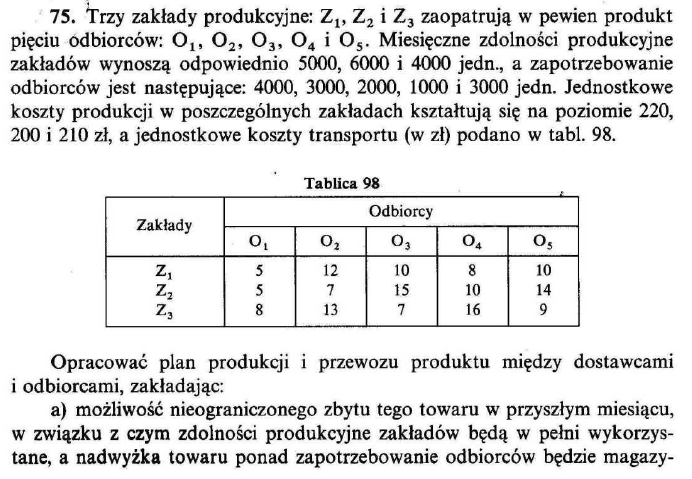
\includegraphics[scale=0.5]{images/obrazek1.png}
    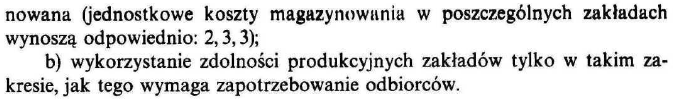
\includegraphics[scale=0.5]{images/obrazek2.png}
  \end{frame}
  \begin{frame}{Optymalizacja}
    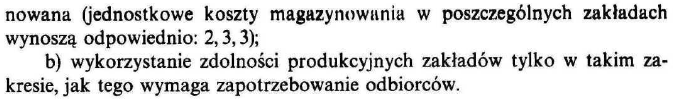
\includegraphics[scale=0.5]{images/obrazek2.png}
    Optymalny plan produkcji okazuje się być taki sam w obu przypadkach: 
    \begin{table}[]
      \begin{tabular}{|l|l|l|l|l|l|l|}
      \hline
         & O1   & O2   & O3   & O4   & O5   & MAGAZYN \\ \hline
      Z1 & 1000 & 0    & 0    & 1000 & 1000 & 2000    \\ \hline
      Z2 & 3000 & 3000 & 0    & 0    & 0    & 0       \\ \hline
      Z4 & 0    & 0    & 2000 & 0    & 2000 & 0       \\ \hline
      \end{tabular}
      \end{table}

  \end{frame}
 
  \begin{frame}{Prawdopodobieństwo}
    Danych jest 5 pudełek ponumerowanych liczbami od 1 do 5. W każdym pudełku znajduje się 20 kul ponumerowanych liczbami od 1 do 20.
    Z każdego pudełka wybieramy jedną kulę. Oblicz prawdopodobieństwo zdarzenia polegającego na tym, że każda z wylosowanych liczb jest
    mniejsza od wszystkich liczb wylosowanych z pudełek o większych numerach oraz suma wylosowanych liczb jest podzielna przez 3.  
    
    Zasymulowana szansa na osiągnięcie powyżej opisanego zdarzenia to 0.1602\% . 
  \end{frame}

  \begin{frame}
    \centering \huge Dziękujemy za uwagę 
  \end{frame}
\end{document}